\section{Verification}\label{sec:results}
The FSM is verified against three-dimensional shell eigenvalue analysis with the same MITC4 flat-facet
Reissner--Mindlin element used throughout OpenSG, on axially-compressed cylinders and a tapered cone. The
walls are (i) isotropic ($E=\SI{200}{\giga\pascal}$, $\nu=0.3$) and (ii) a balanced-symmetric
$[\pm45^\circ]_s$ carbon/epoxy laminate ($E_1=\SI{140}{\giga\pascal}$, $E_2=\SI{10}{\giga\pascal}$,
$G_{12}=\SI{5}{\giga\pascal}$, $\nu_{12}=0.3$), thickness $t=\SI{0.02}{\metre}$. The pre-buckling state is
uniform axial (meridional) compression; the FSM and the shell FEA are driven by the \emph{same} membrane
resultant $\NN$, so the comparison isolates the buckling formulation. The shell FEA uses a refined
circumferential mesh ($n_c=240$); mesh refinement moves the FEA \emph{downward} (coarse meshes over-predict
buckling), so the FSM/FEA ratios below are conservative bounds on the FSM accuracy.

\subsection{Isotropic cylinder}
For $R=\SI{1}{\metre}$, $L=\SI{2}{\metre}$ ($R/t=50$) the classical critical membrane force is
$N_{\mathrm{cr}}^{\mathrm{cl}}=E t^2/[R\sqrt{3(1-\nu^2)}]=\SI{4.842e7}{\newton\per\metre}$. The FSM signature
curve (Fig.~\ref{fig:sig}) drops to a clean plateau at half-wavelength $a\!\approx\!1.7\sqrt{Rt}$ with
minimum $N_{\mathrm{cr}}^{\mathrm{FSM}}=\SI{4.74e7}{\newton\per\metre}$, i.e.\ $0.979\,N_{\mathrm{cr}}^{\mathrm{cl}}$;
the refined three-dimensional shell FEA gives $\SI{4.58e7}{\newton\per\metre}$ ($0.946\,N_{\mathrm{cr}}^{\mathrm{cl}}$),
its small deficit the facet approximation of the curved surface. The FSM thus brackets the exact value more
tightly than the shell FEA and costs $\SI{4.5}{\second}$ against several minutes for the
$\num{174240}$-DOF ($n_c=240$) shell eigenproblem.

\subsection{Anisotropic $[\pm45^\circ]_s$ cylinder: the multi-harmonic recovery}
A single harmonic returns $N_{\mathrm{cr}}=\SI{6.57e6}{\newton\per\metre}$, $1.20\times$ the shell FEA
($\SI{5.47e6}{\newton\per\metre}$): the $20\%$ over-prediction is exactly the bend--twist coupling
$D_{16},D_{26}$ annihilated by \eqref{eq:orth}. Restoring it through the multi-harmonic series
\eqref{eq:series}--\eqref{eq:kcouple} converges the load downward as opposite-parity harmonics couple
(Table~\ref{tab:multi}): from $1.59\times$ at $M{=}1$ to $1.09\times$ by $M{\ge}12$. The isotropic wall,
having no $16/26$ terms to recover, is insensitive to $M$ ($1.016\times$ throughout). Mesh refinement
(circumferential $n_c=160\!\to\!240$) confirms the remaining $[\pm45^\circ]$ gap is not a discretization
artifact of the reference: the three-dimensional shell buckling converges \emph{downward}
($1.088\!\to\!1.109\times$), as coarse meshes over-predict, so the shear-rigid FSM sits genuinely above the
shear-soft shell. The isotropic ratio stays at $\sim\!1.02$---a formulation floor between the analytic strip
and the facet shell that is not transverse shear---while the $[\pm45^\circ]$-specific excess of $\sim\!9\%$
is the transverse-shear flexibility of the $\pm45$ wall, which the present Kirchhoff strip omits. A
Reissner--Mindlin strip (future work) restores it, closing the anisotropic case to within the same
few-percent floor; it is negligible for this thin tube but essential for foam-core sandwich panels.

\begin{table}[h]\centering
\caption{Multi-harmonic convergence of the FSM local buckling load, ratio to the three-dimensional shell
FEA, for the axially-compressed $[\pm45^\circ]_s$ cylinder ($M$ = number of longitudinal harmonics).}
\label{tab:multi}
\begin{tabular}{lcccccc}
\toprule
$M$ & 1 & 4 & 8 & 12 & 16 & 20 \\
\midrule
$N_{\mathrm{cr}}^{\mathrm{FSM}}/N_{\mathrm{cr}}^{\mathrm{FEA}}$ (m45) & 1.594 & 1.562 & 1.104 & 1.089 & 1.088 & 1.088 \\
$N_{\mathrm{cr}}^{\mathrm{FSM}}/N_{\mathrm{cr}}^{\mathrm{FEA}}$ (iso) & 1.016 & 1.016 & 1.016 & 1.016 & 1.016 & 1.016 \\
\bottomrule
\end{tabular}
\end{table}

\begin{figure}[h]\centering
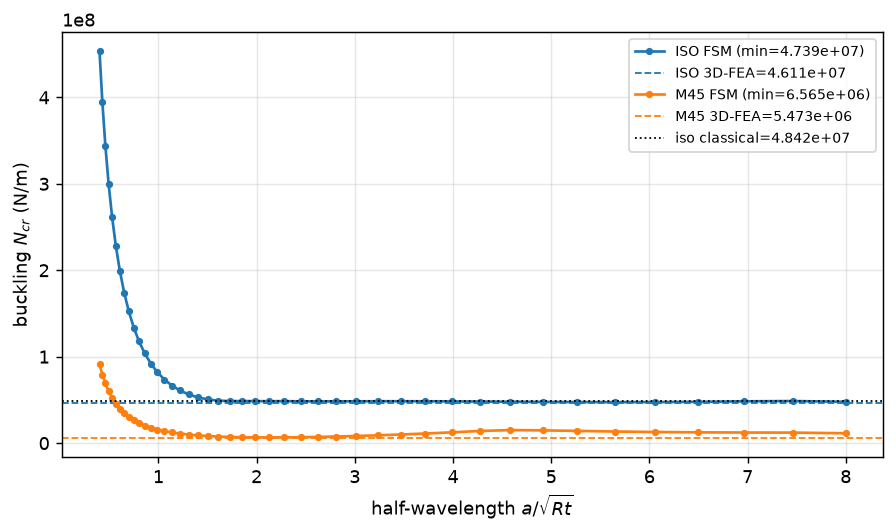
\includegraphics[width=0.72\textwidth]{fig/fsm_cyl_signature.png}
\caption{FSM signature curves (buckling $N_{\mathrm{cr}}$ vs.\ half-wavelength $a/\sqrt{Rt}$) for the
isotropic and $[\pm45^\circ]_s$ cylinders, with the three-dimensional shell FEA (dashed) and the isotropic
classical value (dotted). The minimum of each curve is the local buckling load.}
\label{fig:sig}
\end{figure}

The first two buckling mode shapes are compared between the direct shell FEA and the FSM-RM
reconstruction (cross-section eigenvector times the longitudinal sinusoid). The isotropic cylinder is
\emph{Koiter-degenerate}---a whole family of axial/circumferential wavenumber pairs $(m,n)$ buckles at
essentially the same load, so even the two shell-FEA modes differ in wavenumber---and the two solvers
therefore realize different members of this critical family. Fig.~\ref{fig:modeiso} shows, for each FEA
mode, the FSM member of the same circumferential order $n$ ($n=6$ and $n=5$): both produce the same
short-wave diamond at the same critical load. The $[\pm45^\circ]_s$ wall breaks the degeneracy---its
bend--twist coupling $D_{16}$ selects a \emph{unique} helical buckle---which the multi-harmonic FSM
reproduces directly, matching the shell FEA mode for mode (Fig.~\ref{fig:modem45}).

\begin{figure}[h]\centering
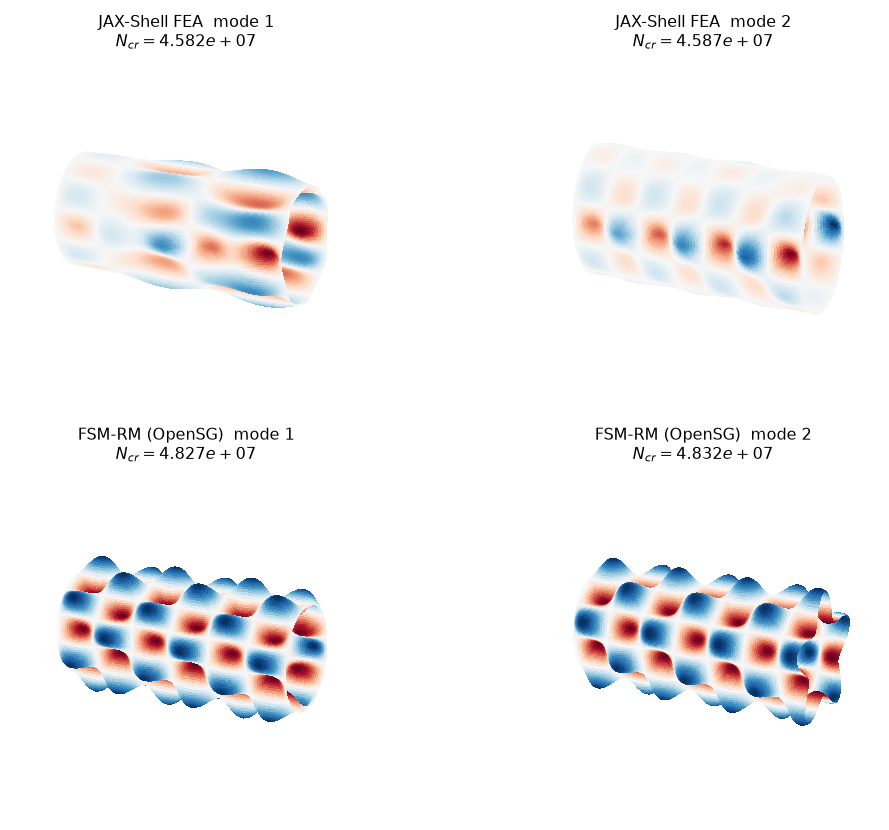
\includegraphics[width=0.82\textwidth]{fig/cyl_iso_modes.png}
\caption{Isotropic cylinder, first two axial local-buckling modes (deformed shape coloured by radial
displacement): JAX-Shell FEA (top) vs.\ FSM-RM/OpenSG (bottom). The cylinder is Koiter-degenerate, so
for each FEA mode the FSM member of matching circumferential order is shown (here $n=6$ and $n=5$);
both are short-wave diamond modes at the same critical load. Refined shell mesh, $n_c=240$.}
\label{fig:modeiso}
\end{figure}

\begin{figure}[h]\centering
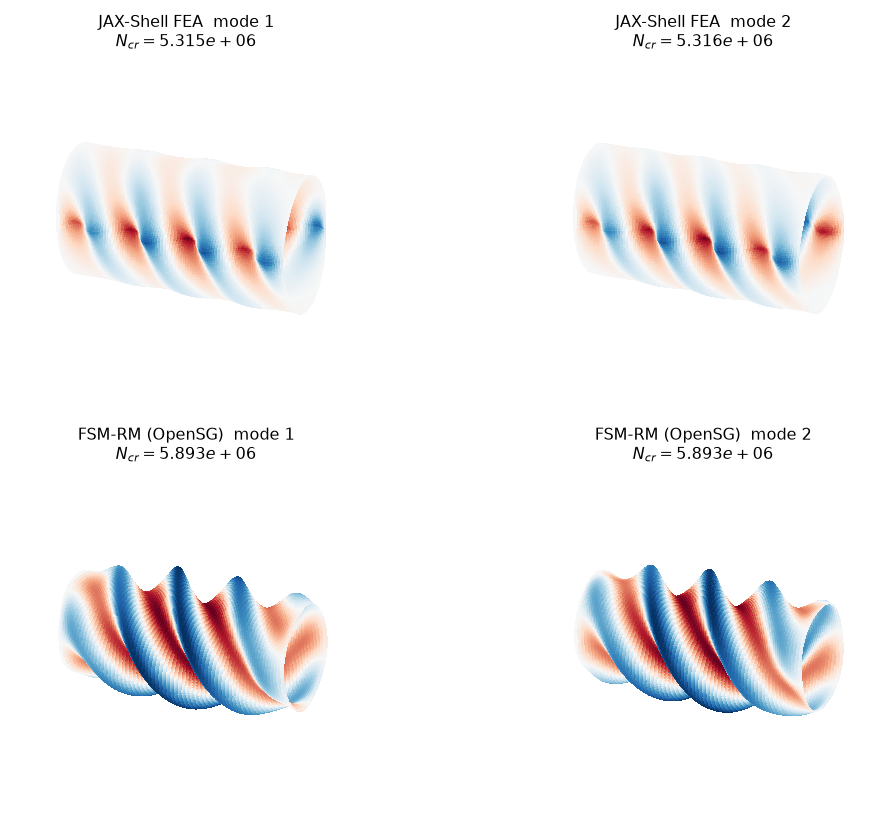
\includegraphics[width=0.82\textwidth]{fig/cyl_m45_modes.png}
\caption{$[\pm45^\circ]_s$ cylinder, first two axial local-buckling modes: JAX-Shell FEA (top) vs.\
FSM-RM/OpenSG (bottom, multi-harmonic reconstruction). The bend--twist coupling tilts the buckle.}
\label{fig:modem45}
\end{figure}

\subsection{Tapered cone: connected and different cross-sections}\label{sec:cone}
The tapered cone ($R_1=\SI{1}{\metre}\!\to\!R_2=\SI{0.5}{\metre}$ over $L=\SI{2}{\metre}$,
$\cos\alpha=0.970$) is the first test of \emph{different} cross-sections along the span. The
\JAXFEA\ buckles the full three-dimensional shell cone; the \RMFSM\ pathway represents the cone by three
cross-sections---root, mid, tip---and takes the minimum FSM factor \eqref{eq:min}. Both are driven by the
analytic meridional pre-stress $N(x)=-P/[2\pi R(x)\cos\alpha]$.

\begin{table}[h]\centering
\caption{Tapered cone axial local buckling: \JAXFEA\ (full 3-D shell) vs.\ \RMFSM\ (minimum over three
cross-sections). Buckling reported as the axial-force factor at bifurcation.}
\label{tab:cone}
\begin{tabular}{lccc}
\toprule
 & \JAXFEA & \RMFSM\ (3-section min) & FSM/FEA \\
\midrule
isotropic cone & $2.668\times10^{8}$ & $2.796\times10^{8}$ & $1.048$ \\
$[\pm45^\circ]_s$ cone & $3.149\times10^{7}$ & $3.539\times10^{7}$ & $1.124$ \\
\bottomrule
\end{tabular}
\end{table}

For both cones the FSM factor is smallest at the \emph{tip} station ($R_2=\SI{0.5}{\metre}$)---the highest
membrane resultant $N\!\propto\!1/R$---so the minimum \eqref{eq:min} correctly localizes the critical
cross-section (isotropic: $2.856,2.886,2.796\times10^{8}$ at $R=1.0,0.75,0.5$; $[\pm45^\circ]$:
$3.630,3.580,3.539\times10^{7}$). The agreement with the full three-dimensional cone
(isotropic $1.048$, $[\pm45^\circ]$ $1.124$) matches the prismatic cylinder to within the same
transverse-shear-limited margin: the per-station representation introduces \emph{no additional error}
beyond the constitutive one, validating the cross-section-based pathway for non-prismatic (blade)
geometries where each station carries a different contour, laminate and pre-buckling stress.
